% Chapter Template

\chapter{System Design and Architecture}\doublespacing % Main chapter title

\label{Chapter5} % Change X to a consecutive number; for referencing this chapter elsewhere, use \ref{ChapterX}

\lhead{Chapter V. \emph{System Design and Architecture}} % Change X to a consecutive number; this is for the header on each page - perhaps a shortened title


% --------------------------------
% Study Summary
% --------------------------------

\section{Introduction}
\noindent The system design and architecture are of utmost importance when it comes to the implementation of a supply chain management system using blockchain technology. A well-designed system ensures the efficient and secure management of the supply chain, leveraging the unique capabilities offered by blockchain.
To effectively design the system architecture for a blockchain-based supply chain management system, several key aspects need to be considered. These include:

% ----------------------------
% Conclusions
% ----------------------------

\subsection{Hyperledger Fabric}
\noindent The Fabric network comprises three organizations (Manufacturer, Middle Men, and Consumer) with five peers, one orderer, and one channel. Each organization has its own Fabric CA for managing digital certificates. The network uses Fabric CA as the Certificate Authority for secure authentication and authorization. The peers maintain a copy of the shared ledger and execute chaincode for smart contracts. The Orderer validates and orders transactions, ensuring consistency. The Fabric network with Fabric CA provides a secure, transparent, and efficient solution for managing the operations.
% \begin{figure}[ht]
\centering
\begin{minipage}[b]{\linewidth}
  \centering
  \includegraphics[width=0.4\linewidth]{Chapters/Chapter_3/figures/Image3_1a.PNG}
  \subcaption{Plot1 with a single image (Image by pencil parker from Pixabay)}
\end{minipage}

\begin{minipage}[b]{\linewidth}
  \centering
  \includegraphics[width=0.4\linewidth]{Chapters/Chapter_3/figures/Image3_1b.PNG}
  \subcaption{Plot2 with a single image (Image by pencil parker from Pixabay)}
\end{minipage}
\caption{Main caption}
\label{fig:figure3_1}
\end{figure}









\begin{figure}[htbp]
  \centering
  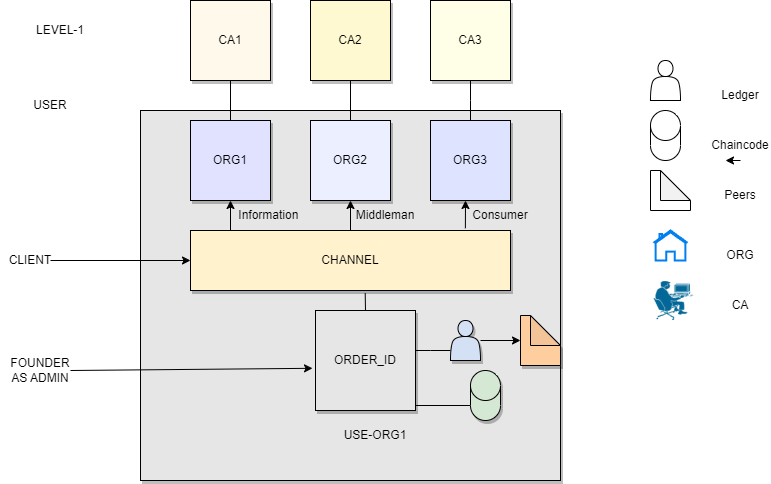
\includegraphics[width=0.9\textwidth]{Chapters/Chapter_5/figures/figure5_1.png}
  \caption{Hyperledger Fabric network Architecture }
  \label{fig:figure5_1}
  \end{figure}

\noindent The Fabric network comprises three organizations (Manufacturer, Middle Men, and Consumer) with five peers, one orderer, 
and one channel. Each organization has its own Fabric CA for managing digital certificates. The network uses Fabric CA as 
the Certificate Authority for secure authentication and authorization. The peers maintain a copy of the shared ledger and 
execute chain code for smart contracts. The Orderer validates and orders transactions, ensuring consistency. The Fabric 
network with Fabric CA provides a secure, transparent, and efficient solution for managing operations.

\begin{itemize}
  \item Admin: all the organization.
  \item Manufacturer: Org1.
  \item Middleman: Org2.
  \item Consumer: Org3.
  
\end{itemize}
    
% ----------------------------
% Scope for Future Work
% ----------------------------

\subsection{Membership and Access Control}
\begin{figure}[htbp]
  \centering
  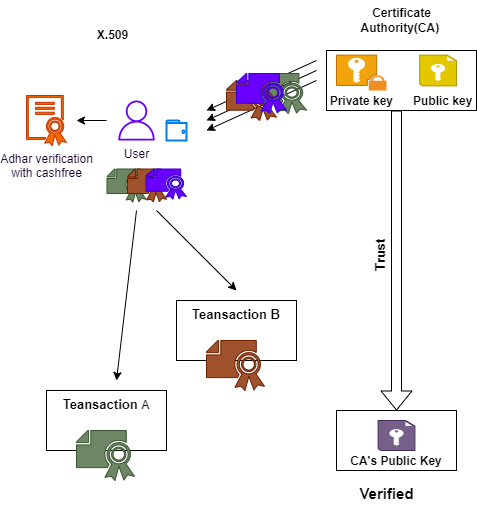
\includegraphics[width=0.9\textwidth]{Chapters/Chapter_5/figures/x.509.png}
  \caption{X.509 Identity Management }
  \label{fig:figure5_2}
  \end{figure}
\noindent \ref{fig:figure5_2} shows that there is a CA that issues a certificate to the user, and this X.059 certificate has multiple attributes whenever 
the user performs a transaction, it signs using this certificate and also checks for Aadhar verification status. Any other entity 
in the system that can view these transactions will be able to see their attributes, thereby knowing that the transaction was 
performed by the particular user to ensure trustworthy of each user in the network.

\subsection{Machine Learning}
\noindent 
The developed solution presents a machine learning (ML) model for detecting the freshness of fruits using a Convolutional Neural Network (CNN) algorithm. The model is trained using TensorFlow, an open-source library for deep learning and machine learning tasks, and is supported by other libraries such as NumPy, Pandas, and Matplotlib for data handling, data cleaning, and visualization. The dataset used for training the model is imported, and its length is verified to be 10901. The model is trained with a sequential model using different layers, including convolutional, activation, dropout, max pooling, flattening, and dense, each serving a specific function in the training process. Keras, a popular library for building neural networks, is used to create the final layers of the CNN model.
\par The model is compiled with the Adamax optimizer, a commonly used optimizer in ML models. During training, the data is traversed multiple times using epochs, with an epoch value of 30 in this case. A validation-data of validation-generator with verbose 1 used and a batch size of 15 is used in the model training process. The proposed approach combines various libraries, algorithms, and tools to develop an ML model for detecting the freshness of fruits based on their condition, which can be beneficial in tracking the quality of products in supply chains. The solution contributes to the expanding body of literature on blockchain applications by providing an effective, dependable, secure, and decentralized trace and track solution using ML and blockchain technologies.
\begin{figure}[ht]
  \centering
  \begin{minipage}[b]{0.4\linewidth}
    \centering
    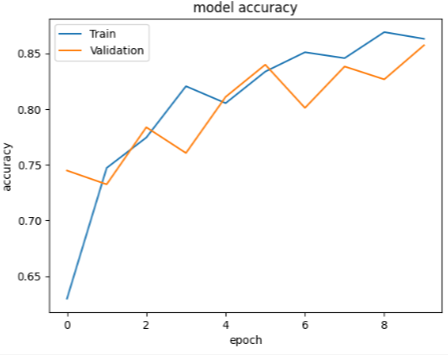
\includegraphics[width=\linewidth]{Chapters/Chapter_5/figures/model_accurecy.png}
    \subcaption{Model Accurecy}
  \end{minipage}
  \hfill
  \begin{minipage}[b]{0.4\linewidth}
    \centering
    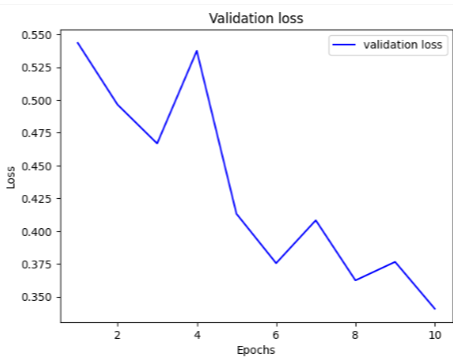
\includegraphics[width=\linewidth]{Chapters/Chapter_5/figures/validationloss.png}
    \subcaption{Validation loss}
  \end{minipage}
  \caption{Main caption}
  \label{fig:figure5_3}
  \end{figure}
  
  % \begin{figure}[ht]
  %   \centering
  %   \begin{minipage}[b]{0.7\linewidth}
  %     \centering
  %     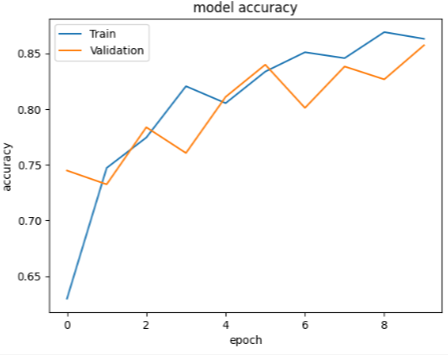
\includegraphics[width=\linewidth]{Chapters/Chapter_5/figures/model_accurecy.png}
  %     \subcaption{Model Accuracy}
  %   \end{minipage}
  
  %   \vspace{0.5cm} % Adjust the vertical space between the images
  
  %   \begin{minipage}[b]{0.4\linewidth}
  %     \centering
  %     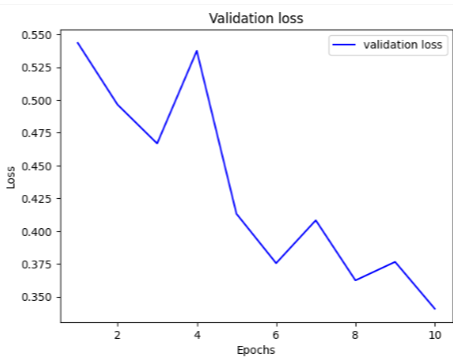
\includegraphics[width=\linewidth]{Chapters/Chapter_5/figures/validationloss.png}
  %     \subcaption{Validation Loss}
  %   \end{minipage}
    
  %   \caption{Main Caption}
  %   \label{fig:figure5_3}
  % \end{figure}
  
  
  
  
  
  
  
\noindent \ref{fig:figure5_3} (a) shows the training accuracy and Validation accucy.Train graph shows the overall model’s Training accuracy and validation accuracy shows the Subset of the training data .It is seen that with each epoch Model is giving more accuracy also validation accuracy too. Validation accuracy is calculated by using subset of the whole 
Training dataset.The final accuracy of the Model is found to be 88.5\%.
\ref{fig:figure5_3} (b) shows the output result that our model  provides.It can be seen That our model is providing us the correct
output.For a rotten Fruit it predicts the fruit as rotten and for a fresh it predicts as fresh.



